\documentclass[sigconf]{acmart}

% --- Additional Mathematical & Formatting Packages ---
\usepackage{booktabs}
\usepackage{multirow}
\usepackage{amsmath,amsfonts}
\usepackage{tikz}
\usepackage{pgfplots}
\usepackage{url}
\usepackage{xurl}

\emergencystretch=1.5em


\pgfplotsset{compat=1.18}
\usetikzlibrary{shapes.geometric, arrows.meta, positioning, calc, backgrounds, fit}

% Suppress ACM Reference Format and Copyright block for Review / Submission draft
\settopmatter{printacmref=false}
\renewcommand\footnotetextcopyrightpermission[1]{}
\pagestyle{plain}

% ACM Rights & Conference Metadata for ICIIT 2027
\setcopyright{none}
\acmConference[ICIIT 2027]{2027 12th International Conference on Intelligent Information Technology}{March 04--07, 2027}{Ho Chi Minh City, Vietnam}
\acmYear{2027}
\copyrightyear{2027}
\acmDOI{}
\acmISBN{}

\begin{document}

\title[Benchmarking Inverse Reasoning and Tabular Transformation Discovery in Frontier LLMs]{Benchmarking Inverse Reasoning and Tabular Transformation Discovery in Frontier Large Language Models: A Two-Tier Autonomous Evaluation Harness}

\author{Viet Dao}
\affiliation{%
  \institution{FPT University}
  \city{Hanoi}
  \country{Vietnam}
}
\email{daothevietnb123@gmail.com}

\begin{abstract}
Reverse engineering the latent data-generating mechanisms of tabular datasets is a fundamental inverse problem that challenges inductive reasoning, automated feature engineering, and programmatic comprehension in artificial intelligence. While Large Language Models (LLMs) demonstrate remarkable proficiency in forward mathematical reasoning and code synthesis, their capacity to infer, isolate, and reconstruct hidden parametric transformation pipelines solely from observational input-output data tables remains underexplored. In this work, we present the \textbf{Tabular Transformation Discovery Harness}, an autonomous, two-tier evaluation framework designed to benchmark LLM agents on inverse tabular induction across six standardized structural complexity classes (from Class 0: Atomic Unary to Class 5: Deep Hybrid ASTs) spanning eight diverse real-world domains. The harness enforces strict epistemic isolation: an agentic discovery phase operating in an iterative, sandbox Read-Eval-Print Loop (REPL) environment with adaptive resource budgets is decoupled from an independent, black-box functional evaluation phase on hidden holdout distributions. In the REPL sandbox, the agent iteratively tests candidate Python transformations, inspects execution output, and refines mathematical hypotheses under hard budget constraints. We conduct extensive empirical evaluations comparing frontier coding and multimodal agents (Claude 3.5 Sonnet, Gemini 3 Flash), a lightweight edge reasoning model (GPT-5.4 Nano), and an exhaustive combinatorial baseline across 48 standardized benchmark tasks ($N=48$, 8 datasets $\times$ 6 complexity classes in a balanced full-factorial design). Our empirical findings reveal a pronounced divergence across paradigms: while Claude 3.5 Sonnet achieves a 70.8\% submission rate with 0.811 conditional transformed accuracy (0.575 penalized accuracy), Gemini 3 Flash achieves 0.844 conditional transformed accuracy but exhibits an over-conservative stopping policy (50.0\% submission rate, 0.422 penalized accuracy). GPT-5.4 Nano achieves 100\% submission but suffers a steep monotonic degradation from 1.000 on Class 0 to 0.250 on Class 5, and depth-3 combinatorial brute-force enumeration collapses on deep interaction graphs (0.375). Furthermore, through a three-mode ablation study, we demonstrate that direct symbolic generation without execution feedback fails almost entirely (3.6\% accuracy), whereas revealing oracle operator vocabularies yields perfect 100\% conditional functional recovery on submitted tasks (66.7\% penalized accuracy). This demonstrates that while programmatic compilation from known operators is highly reliable in frontier models, hypothesis search under observational uncertainty and budget-constrained stopping heuristics remain the primary operational bottlenecks. All code, benchmark tasks, and evaluation harnesses are made open-source at \url{https://github.com/mini-smart-lab/tabular-transformation}.
\end{abstract}

\begin{CCSXML}
<ccs2012>
   <concept>
       <concept_id>10010147.10010178.10010187</concept_id>
       <concept_desc>Computing methodologies~Knowledge representation and reasoning</concept_desc>
       <concept_significance>500</concept_significance>
   </concept>
   <concept>
       <concept_id>10010147.10010257</concept_id>
       <concept_desc>Computing methodologies~Machine learning</concept_desc>
       <concept_significance>500</concept_significance>
   </concept>
   <concept>
       <concept_id>10011007.10011074.10011099</concept_id>
       <concept_desc>Software and its engineering~Software verification and validation</concept_desc>
       <concept_significance>300</concept_significance>
   </concept>
</ccs2012>
\end{CCSXML}

\ccsdesc[500]{Computing methodologies~Knowledge representation and reasoning}
\ccsdesc[500]{Computing methodologies~Machine learning}
\ccsdesc[300]{Software and its engineering~Software verification and validation}

\keywords{Tabular Data, Inverse Program Induction, Large Language Models, Autonomous Agent, Two-Tier Evaluation Harness, Symbolic Recovery}

\maketitle

\section{Introduction}

Tabular data remains the predominant data modality in mission-critical industrial, scientific, and financial domains~\cite{borisov2022deep,grinsztajn2022tree}. Despite the recent ascendancy of Large Language Models (LLMs) across natural language and software engineering domains~\cite{achiam2023gpt4,anthropic2024claude35,geminiteam2024gemini,jimenez2024swebench}, tabular data structures present unique fundamental challenges: permutation-invariant columns, heterogeneous distributions, non-linear cross-column correlations, and rigid numerical dependencies that cannot be inferred purely via autoregressive token modeling~\cite{xu2019synthesizing,kotelnikov2023tabddpm,sui2024table}.

A central challenge at the intersection of automated machine learning and program synthesis is \emph{inverse tabular transformation reasoning}: given an observational baseline dataset $\mathcal{D}_{\text{before}}$ and an engineered or transformed dataset $\mathcal{D}_{\text{after}}$, can an autonomous AI agent infer, formulate, and execute the exact latent programmatic transformation $\mathcal{T}$ such that $\mathcal{T}(\mathcal{D}_{\text{before}}) \approx \mathcal{D}_{\text{after}}$? Developing this capability is critical for auditing and reverse-engineering legacy ETL (Extract, Transform, Load) pipelines that lack documentation, automating feature discovery in predictive modeling~\cite{cranmer2020frontier}, reconstructing scientific equations from observational physical tables~\cite{schmidt2009distilling,udrescu2020ai}, and identifying potential data privacy leakage in synthetic anonymization protocols~\cite{stadler2022synthetic}.

While popular benchmark suites such as HumanEval~\cite{chen2021evaluating} and SWE-bench~\cite{jimenez2024swebench} evaluate \emph{forward} reasoning—where formal specifications or natural language descriptions dictate desired program semantics—inverse tabular induction requires \emph{scientific hypothesis formation under uncertainty}. The agent operates in a Read-Eval-Print Loop (REPL) environment—an interactive programming shell where candidate code snippets are executed immediately in an isolated interpreter, returning runtime stdout, stderr, and numerical summaries to guide subsequent reasoning. Within this REPL paradigm, the agent must:
\begin{enumerate}
    \item Inspect multivariate numeric distributions across high-dimensional feature spaces;
    \item Disentangle candidate mathematical hypotheses (e.g., distinguishing logarithmic scaling from power-law decays or piecewise segmentations);
    \item Interactively experiment using executable code in the sandboxed REPL;
    \item Synthesize a clean, self-contained, parametric Python function $\texttt{transform}(\texttt{df})$ that generalizes out-of-distribution.
\end{enumerate}

Prior benchmarks attempting to evaluate programmatic reasoning suffer from critical methodological shortcomings. First, many rely on synthetic toy distributions (e.g., uniform or normal random variables) rather than authentic tabular benchmarks, ignoring the multi-collinearity, skewed kurtosis, and boundary anomalies inherent in empirical datasets. Second, existing evaluation frameworks often execute candidate solutions in the same environment where test data resides, introducing severe risks of data leakage and contamination. Third, standard evaluation metrics frequently conflate \emph{code generation accuracy} with \emph{hypothesis search efficiency}, making it impossible to diagnose whether an agent failed because it could not discover the underlying mathematical law or because it made a trivial syntactic error during program synthesis.

\begin{figure*}[t!]
\centering
\resizebox{0.88\textwidth}{!}{
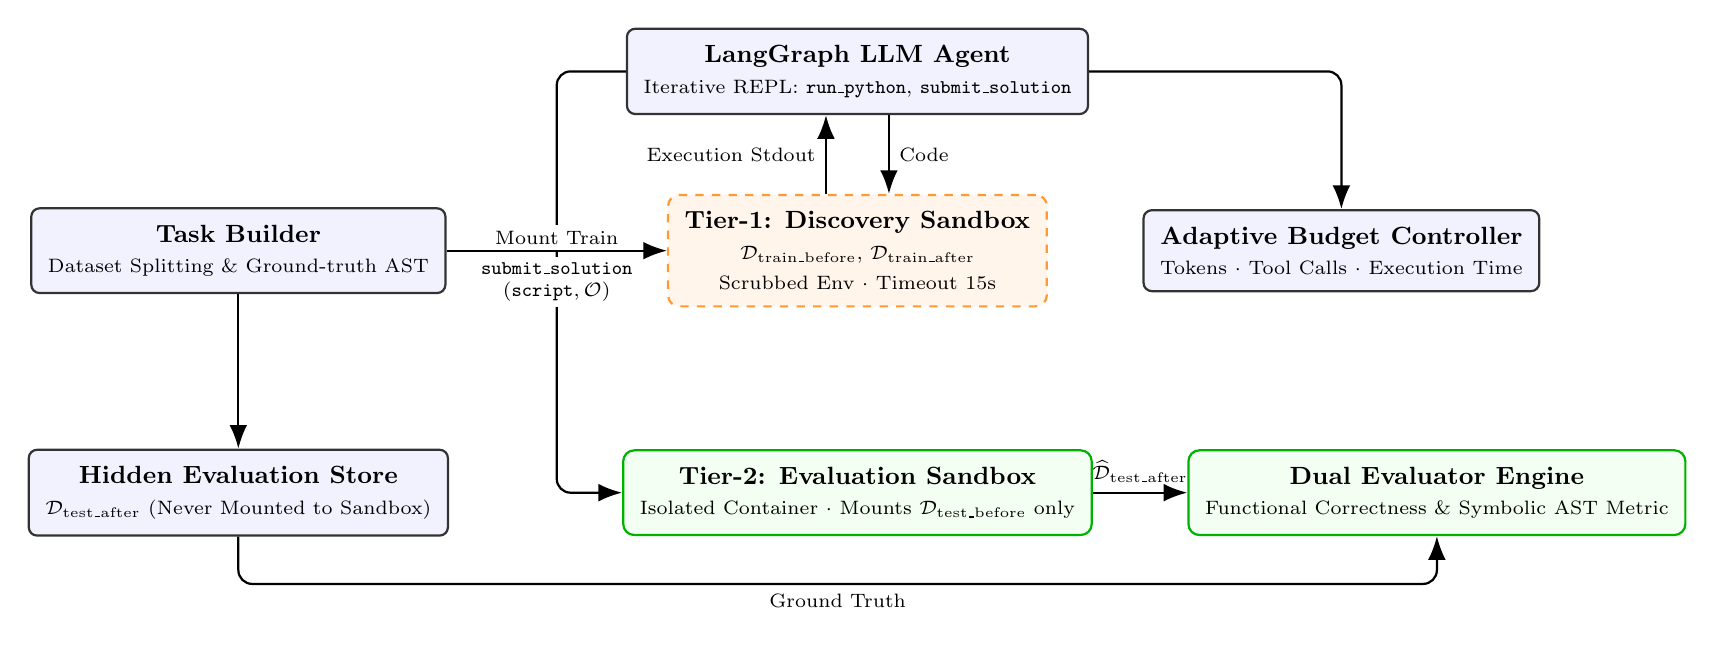
\begin{tikzpicture}[
    node distance=1.4cm and 1.6cm,
    box/.style={rectangle, draw=black!80, fill=blue!5, rounded corners=3pt, thick, align=center, inner sep=6pt, font=\small},
    sand/.style={rectangle, draw=orange!80, fill=orange!8, rounded corners=4pt, dashed, thick, align=center, inner sep=6pt, font=\small},
    eval/.style={rectangle, draw=green!70!black, fill=green!5, rounded corners=4pt, thick, align=center, inner sep=6pt, font=\small},
    arrow/.style={-{Latex[length=3mm]}, thick}
]

% Tier 1: Task Gen & Discovery
\node[box] (taskgen) {\textbf{Task Builder}\\\scriptsize Dataset Splitting \& Ground-truth AST};
\node[sand, right=2.8cm of taskgen] (sand1) {\textbf{Tier-1: Discovery Sandbox}\\\scriptsize $\mathcal{D}_{\text{train\_before}}$, $\mathcal{D}_{\text{train\_after}}$\\\scriptsize Scrubbed Env $\cdot$ Timeout 15s};
\node[box, above=1cm of sand1] (agent) {\textbf{LangGraph LLM Agent}\\\scriptsize Iterative REPL: \texttt{run\_python}, \texttt{submit\_solution}};
\node[box, right=1.2cm of sand1] (budget) {\textbf{Adaptive Budget Controller}\\\scriptsize Tokens $\cdot$ Tool Calls $\cdot$ Execution Time};

% Tier 2: Independent Evaluation
\node[eval, below=1.8cm of sand1] (sand2) {\textbf{Tier-2: Evaluation Sandbox}\\\scriptsize Isolated Container $\cdot$ Mounts $\mathcal{D}_{\text{test\_before}}$ only};
\node[eval, right=1.2cm of sand2] (evaluator) {\textbf{Dual Evaluator Engine}\\\scriptsize Functional Correctness \& Symbolic AST Metric};
\node[box] (hiddendata) at (taskgen |- sand2) {\textbf{Hidden Evaluation Store}\\\scriptsize $\mathcal{D}_{\text{test\_after}}$ (Never Mounted to Sandbox)};

% Paths
\draw[arrow] (taskgen) -- (hiddendata);
\draw[arrow] ([xshift=0.4cm]agent.south) -- node[right, font=\scriptsize]{Code} ([xshift=0.4cm]sand1.north);
\draw[arrow] ([xshift=-0.4cm]sand1.north) -- node[left, font=\scriptsize]{Execution Stdout} ([xshift=-0.4cm]agent.south);
\draw[arrow, rounded corners=5pt] (agent.east) -| (budget.north);

\path (taskgen.east) -- (sand1.west) coordinate[midway] (midgap);
\draw[arrow, rounded corners=5pt] (agent.west) -- (midgap |- agent.west) -- node[fill=white, align=center, font=\scriptsize, inner sep=2pt]{$\texttt{submit\_solution}$\\$(\texttt{script}, \mathcal{O})$} (midgap |- sand2.west) -- (sand2.west);
\draw[arrow] (taskgen) -- node[above, fill=white, inner sep=2pt, font=\scriptsize]{Mount Train} (sand1);
\draw[arrow] (sand2) -- node[above, font=\scriptsize]{$\widehat{\mathcal{D}}_{\text{test\_after}}$} (evaluator);

\path (hiddendata.south) -- ++(0, -0.6) coordinate (bot);
\draw[arrow, rounded corners=5pt] (hiddendata.south) -- (hiddendata.south |- bot) -- node[below, font=\scriptsize]{Ground Truth} (evaluator.south |- bot) -- (evaluator.south);

\end{tikzpicture}
}
\caption{Two-Tier Evaluation Harness Architecture. Tier 1 provides an isolated REPL discovery environment with sanitized environment variables, strictly bounded by the Adaptive Budget Controller. Tier 2 performs black-box functional evaluation on hidden holdout distributions without network access or host secret exposure.}
\label{fig:two_tier_arch}
\end{figure*}

To overcome these fundamental limitations, we propose the \textbf{Tabular Transformation Discovery Harness}, a rigorous research framework featuring:
\begin{enumerate}
    \item \textbf{A Formal Taxonomy of 6 Structural Complexity Classes:} Ranging from atomic unary operations (Class 0) to deep hybrid Abstract Syntax Trees (ASTs) containing piecewise conditionals and multi-column interactions (Class 5).
    \item \textbf{A Two-Tier Epistemic Isolation Architecture:} Tier 1 provides an interactive REPL discovery sandbox where the agent executes arbitrary Python code on training split pairs $(\mathcal{D}_{\text{train\_before}},$ $\mathcal{D}_{\text{train\_after}})$, governed by an Adaptive Tiered Budget Controller. Tier 2 executes the submitted script in a fresh container on an unobserved holdout set $\mathcal{D}_{\text{test\_before}}$, strictly isolated from $\mathcal{D}_{\text{test\_after}}$ (Figure~\ref{fig:two_tier_arch}).
    \item \textbf{A Multi-Domain Benchmark Suite Across 8 Real-World Datasets ($N=48$ Tasks):} Sourced from diverse domains (aeronautics, clinical medicine, civil engineering, computer systems telemetry, food chemistry, oncology, economics, and security signal processing), compiled into a balanced full-factorial design across all 6 complexity classes (8 datasets $\times$ 6 classes = 48 tasks).
    \item \textbf{A Cross-Paradigm Empirical Study:} Benchmarking a frontier coding agent (Claude 3.5 Sonnet), a frontier multimodal agent (Gemini 3 Flash), a lightweight edge reasoning model (GPT-5.4 Nano), and an exhaustive depth-3 combinatorial enumeration baseline.
    \item \textbf{A Rigorous 3-Mode Ablation Protocol:} Isolating the relative contributions of direct parametric reasoning (no tools), interactive hypothesis testing via REPL, and oracle operator disclosure.
\end{enumerate}

All code, benchmark datasets, and evaluation harnesses are publicly available at \url{https://github.com/mini-smart-lab/tabular-transformation}.

\section{Related Work}

\subsection{Tabular Representation Learning and LLMs}
Tabular data presents distinct challenges for deep neural networks due to heterogeneous column distributions, non-spatial correlation, and varying sparsity~\cite{borisov2022deep,grinsztajn2022tree}. While gradient-boosted decision trees (XGBoost, LightGBM) historically dominated supervised tabular benchmarks, recent research has explored adapting deep foundation models and LLMs to tabular structures. Early efforts serialized tabular rows into natural language prompts (TabLLM~\cite{hegselmann2023tabllm}) or instruction-tuned models for structured tables (Table-GPT~\cite{li2024tablegpt}, Sui et al.~\cite{sui2024table}). More recently, scalable tabular foundation models based on In-Context Learning (ICL)—such as TabICL~\cite{qu2025tabicl} and TabICLv2~\cite{qu2026tabiclv2}—employ specialized two-stage architectures with column-then-row attention mechanisms capable of performing in-context prediction across large tabular samples. 

However, all these existing foundation models operate exclusively in the \emph{forward} predictive regime: given observed training examples, predict target labels for test instances. In contrast, our work investigates \emph{inverse program induction}: given observational table pairs before and after transformation, the model must explicitly infer, formalize, and synthesize the latent mathematical code pipeline that generated the transformed data.

\subsection{Program Synthesis and Symbolic Regression}
Symbolic regression aims to uncover closed-form mathematical equations that explain empirical observations~\cite{schmidt2009distilling,udrescu2020ai,cranmer2020frontier}. Genetic programming~\cite{schmidt2009distilling}, AI Feynman~\cite{udrescu2020ai}, and modern evolutionary symbolic regression packages such as PySR~\cite{cranmer2023pysr} utilize Pareto-optimal evolutionary search and physics-inspired modular decomposition to avoid exhaustive combinatorial enumeration. More recently, equation discovery frameworks (e.g., LLM-SR~\cite{shojaee2025llmsr}, LLM-SRBench~\cite{shojaee2025llmsrbench}) prompt LLMs to discover mathematical relationships via program search. In program synthesis, enumerative and deductive techniques infer programs satisfying input-output specifications~\cite{gulwani2017program}. However, classical discrete program synthesis fails to scale to continuous, non-linear tabular transformations involving high-dimensional feature interactions.

\subsection{Autonomous LLM Agents and Execution Sandboxes}
Recent advances in agentic AI combine language model reasoning with external tool execution via iterative ReAct loops~\cite{yao2023react,langgraph2024,madaan2023selfrefine}. In data science, benchmarks such as DS-1000~\cite{lai2023ds1000}, DA-Code~\cite{huang2024dacode}, and feature engineering benchmarks such as FeatEng~\cite{pietruszka2025feateng} evaluate LLMs on forward code synthesis for tabular data manipulation. In software engineering, benchmarks like SWE-bench~\cite{jimenez2024swebench} evaluate autonomous patch generation in repository sandboxes. However, code generation in data science benchmarks relies heavily on natural language prompts or issue descriptions. In contrast, tabular transformation discovery requires unguided inductive hypothesis search from raw numerical arrays without natural language hints.

\section{Problem Formulation and Methodology}

\subsection{Formalization of Tabular Inverse Reasoning}
Let $\mathcal{X} \subseteq \mathbb{R}^M$ denote the feature space of an initial tabular dataset $\mathcal{D}_{\text{before}} = \{\mathbf{x}^{(i)}\}_{i=1}^N \in \mathbb{R}^{N \times M}$ with column schema $\mathcal{C}_{\text{before}} = \{c_1, \dots, c_M\}$. Let $\mathcal{T} : \mathbb{R}^M \to \mathbb{R}^P$ be a deterministic, parameterized transformation mapping:
\begin{equation}
    \mathcal{D}_{\text{after}} = \mathcal{T}(\mathcal{D}_{\text{before}}) \in \mathbb{R}^{N \times P}
\end{equation}
with transformed schema $\mathcal{C}_{\text{after}} = \{\tilde{c}_1, \dots, \tilde{c}_P\}$. 

The transformation pipeline $\mathcal{T}$ is composed of a sequence of operators drawn from a discrete vocabulary of 24 canonical operators $\Omega = \{\omega_1, \dots, \omega_{24}\}$:
\begin{equation}
    \mathcal{T} = \tau_K \circ \tau_{K-1} \circ \dots \circ \tau_1
\end{equation}
where each operator $\tau_k$ is drawn from canonical operations including unary functions (e.g., $\ln(x+1)$, $\sqrt{x}$, $x^2$, $x^3$, $1/x$, $e^x$), trigonometric transforms ($\sin$, $\cos$, $\tanh$), stateful scalers ($\text{StandardScaler}$, $\text{MinMaxScaler}$), bivariate cross-column interactions ($x_i \star x_j$ with $\star \in \{+, -, \times, \div\}$), or piecewise conditionals ($\mathbf{1}_{\{x > \theta\}} \cdot x$).

\noindent\textbf{Parameterization of Stateful Scalers:} For distribution-level operators ($\text{StandardScaler}$, $\text{MinMaxScaler}$), empirical moments ($\mu$, $\sigma^2$, $\min$, $\max$) are fitted solely on $\mathcal{D}_{\text{train\_before}}$. In Tier 2 evaluation, the synthesized $\texttt{transform}(\texttt{df})$ script applies these frozen scalar constants directly to $\mathcal{D}_{\text{test\_before}}$, ensuring mathematically sound out-of-sample functional testing without test-set distributional leakage.

The dataset is partitioned into an observed training split $\mathcal{D}_{\text{train}} = (\mathcal{D}_{\text{train\_before}},$ $\mathcal{D}_{\text{train\_after}})$ of size $N_{\text{train}}$ and a hidden holdout test split $\mathcal{D}_{\text{test}} = (\mathcal{D}_{\text{test\_before}},$ $\mathcal{D}_{\text{test\_after}})$ of size $N_{\text{test}}$, such that $\mathcal{D}_{\text{train}} \cap \mathcal{D}_{\text{test}} = \emptyset$.

\noindent\textbf{The Objective:} Given access solely to $\mathcal{D}_{\text{train\_before}}$ and $\mathcal{D}_{\text{train\_after}}$, an agent must discover and submit an executable Python program $\widehat{\mathcal{T}}$ that minimizes the out-of-sample functional discrepancy:
\begin{equation}
    \min_{\widehat{\mathcal{T}}} \; \mathbb{E}_{\mathbf{x} \sim \mathcal{D}_{\text{test\_before}}} \left[ \|\widehat{\mathcal{T}}(\mathbf{x}) - \mathcal{T}(\mathbf{x})\|_\infty \right]
\end{equation}
while simultaneously recovering the symbolic operator sequence $\widehat{\mathcal{O}} \subseteq \Omega$ that generated the transformations.

\subsection{Six Structural Complexity Classes}
To systematically analyze model reasoning limits, we formalize six structural complexity classes of increasing mathematical depth:
\begin{itemize}
    \item \textbf{Class 0 (Atomic Unary):} Exactly one column is modified by a single primitive operation $y = f(x)$, where $f$ is drawn from unary primitives such as $\text{Square}$, $\text{Sqrt}$, $\text{Exp}$, $\text{Log1p}$, $\text{MinMaxScaler}$, or $\text{Sin}$.
    \item \textbf{Class 1 (Independent Unary):} Multiple columns are modified concurrently by distinct, uncomposed unary transformations: $y_j = f_j(x_j)$ for $j \in \{1, \dots, k\}$.
    \item \textbf{Class 2 (Composed Chains):} Columns undergo sequential compositions of operations, e.g., $y = f_2(f_1(x))$, requiring the agent to identify intermediate latent variables and resolve operator ordering.
    \item \textbf{Class 3 (Multi-Column Interactions):} A new column is generated via binary arithmetic or non-linear interaction between two distinct columns: $z = x_i \star x_j$ with $\star \in \{+, -, \times, \div\}$.
    \item \textbf{Class 4 (Piecewise / Conditional Logic):} Non-linear piecewise segmentation or indicator transformations:
    \begin{equation}
        y = \begin{cases} f_1(x) & \text{if } x > \theta \\ f_2(x) & \text{otherwise} \end{cases}
    \end{equation}
    requiring the agent to identify both the splitting threshold $\theta$ and the branch operations.
    \item \textbf{Class 5 (Deep Hybrid AST):} A Directed Acyclic Graph (DAG) combining multi-step compositions, cross-column interactions, and conditional logic within a single unified feature pipeline.
\end{itemize}

\subsection{Two-Tier Epistemic Isolation Harness}
To eliminate data contamination and host security vulnerabilities, our harness implements a two-tier architectural isolation (Figure~\ref{fig:two_tier_arch}):

\subsubsection{Tier 1: Agentic Discovery Sandbox}
The agent interacts with an isolated Python execution environment via three LangChain-compatible tools:
\begin{itemize}
    \item $\texttt{run\_python}(\texttt{code})$: Acts as an interactive Read-Eval-Print Loop (REPL). The agent executes exploratory data analysis, computes summary statistics, fits regressions, tests candidate operator hypotheses on training tables, generates diagnostic plots, and inspects stdout/stderr feedback. Execution runs in a sanitized subprocess with stripped host environment variables ($\texttt{API\_KEY}$, $\texttt{TOKEN}$) and an enforced 15-second timeout.
    \item $\texttt{read\_image}(\texttt{path})$: Inspects visual charts (e.g., scatter plots, residual distribution curves) saved in the sandbox workspace. The image is loaded directly into the multimodal LLM context, enabling visual pattern recognition of non-linear trends and piecewise thresholds.
    \item $\texttt{submit\_solution}(\texttt{script}, \mathcal{O})$: Formally terminates the discovery phase by submitting a standalone Python script containing a function $\texttt{transform}(\texttt{df})$ and a list of identified symbolic operators $\mathcal{O}$.
\end{itemize}

\subsubsection{Adaptive Tiered Budget Controller}
To prevent infinite reasoning loops and simulate real-world compute budgets, the discovery phase is regulated by an adaptive budget scaled dynamically across complexity classes $c \in \{0, \dots, 5\}$:
\begin{align}
    T_{\text{calls}}(c) &\in [8, 10, 14, 18, 24, 30], \\
    K_{\text{tokens}}(c) &\in [60\text{k}, 80\text{k}, 120\text{k}, 160\text{k}, 220\text{k}, 300\text{k}], \\
    \Delta t_{\text{wall}}(c) &\in [120\text{s}, 120\text{s}, 180\text{s}, 240\text{s}, 300\text{s}, 360\text{s}].
\end{align}

\subsubsection{Tier 2: Independent Evaluation Sandbox}
Upon submission, the harness launches a completely isolated Tier 2 evaluation container. Epistemic isolation is enforced primarily by filesystem unmounting and OS-level network isolation: the ground-truth test target $\mathcal{D}_{\text{test\_after}}$ is stored securely in host memory and is never mounted to any sandbox container. As an additional defense-in-depth barrier, the submitted script is verified via Abstract Syntax Tree (AST) validation for dangerous system calls (such as $\texttt{os.system}$, $\texttt{subprocess}$, or network sockets) before executing on $\mathcal{D}_{\text{test\_before}}$ to generate predicted table $\widehat{\mathcal{D}}_{\text{test\_after}}$.


\subsection{Evaluation Metrics}
We assess performance across two orthogonal dimensions: functional numerical execution and symbolic structural recovery. Importantly, we formalize both \emph{conditional} and \emph{penalized} metrics to address non-submission failure modes.

\subsubsection{Black-Box Functional Metrics}
Let $\mathcal{C}_{\text{after}}$ denote the target column schema. For column $c \in \mathcal{C}_{\text{after}}$, the column match accuracy over $N_{\text{test}}$ rows is:
\begin{equation}
    m(c) = \frac{1}{N_{\text{test}}} \sum_{i=1}^{N_{\text{test}}} \mathbf{1}_{\left\{ |\widehat{D}_{i, c} - D_{i, c}| < \epsilon \cdot (|D_{i, c}| + 1) \right\}}
\end{equation}
with numerical tolerance $\epsilon = 10^{-4}$. Missing, non-finite ($\texttt{NaN}$, $\texttt{Inf}$), or unaligned columns receive $m(c) = 0$. A column is marked correct if $m(c) \ge 0.99$. We compute:
\begin{itemize}
    \item \textbf{Transformed Column Accuracy ($\text{Acc}_{\text{trans}}$):} The fraction of truly transformed columns $\mathcal{C}_{\text{trans}} \subseteq \mathcal{C}_{\text{after}}$ correctly predicted:
    \begin{equation}
        \text{Acc}_{\text{trans}} = \frac{1}{|\mathcal{C}_{\text{trans}}|} \sum_{c \in \mathcal{C}_{\text{trans}}} \mathbf{1}_{\{m(c) \ge 0.99\}}
    \end{equation}
    \item \textbf{Functional Column Accuracy ($\text{Acc}_{\text{func}}$):} The overall fraction of all columns in $\mathcal{C}_{\text{after}}$ (including unmodified columns) correctly predicted across the table.
\end{itemize}

\subsubsection{Conditional vs. Penalized Accuracy}
An agent may exhaust its allocated tool budget or execution timeout without executing $\texttt{submit\_solution}$. To ensure transparent, uninflated evaluation:
\begin{itemize}
    \item \textbf{Conditional Accuracy} ($\text{Acc}_{\text{cond}}$): Metrics calculated strictly across the subset of tasks where the agent explicitly submitted a solution. This quantifies the model's reasoning precision when it commits to a hypothesis.
    \item \textbf{Penalized Accuracy} ($\text{Acc}_{\text{pen}}$): Any task where the agent fails to submit within budget receives a score of \textbf{0}. Formally:
    \begin{equation}
    \begin{split}
        \text{Acc}_{\text{pen}} &= \frac{1}{N_{\text{total}}} \sum_{i=1}^{N_{\text{total}}} \mathbf{1}_{\{\text{submitted}_i\}} \cdot \text{Acc}_i \\
        &= \text{Submission Rate} \times \text{Acc}_{\text{cond}}
    \end{split}
    \end{equation}
\end{itemize}
Evaluating both perspectives prevents models with low submission rates from appearing artificially superior due to selective submission.

\subsubsection{White-Box Symbolic Metrics}
We parse the submitted script into an AST and extract the executed mathematical operator sequence $\widehat{\mathcal{O}}$. Compared against ground truth $\mathcal{O}^*$, we compute:
\begin{itemize}
    \item \textbf{Operator F1 Score ($\text{F1}_{\text{op}}$):} The harmonic mean of operator precision and recall over multiset elements:
    \begin{equation}
        \text{Precision} = \frac{|\widehat{\mathcal{O}} \cap \mathcal{O}^*|}{|\widehat{\mathcal{O}}|}, \quad \text{Recall} = \frac{|\widehat{\mathcal{O}} \cap \mathcal{O}^*|}{|\mathcal{O}^*|}
    \end{equation}
    \item \textbf{Exact Sequence Accuracy ($\text{Acc}_{\text{seq}}$):} Measured at the column level as the fraction of transformed columns where the full composition operator sequence is recovered in identical order:
    \begin{equation}
        \text{Acc}_{\text{seq}} = \frac{1}{|\mathcal{C}_{\text{trans}}|} \sum_{c \in \mathcal{C}_{\text{trans}}} \mathbf{1}_{\{\widehat{\mathcal{O}}_c = \mathcal{O}^*_c\}}
    \end{equation}
\end{itemize}

\section{Experimental Setup}

\subsection{Benchmark Task Construction}
To satisfy stringent real-world validity requirements, we compiled 48 standardized benchmark tasks ($N=48$) sourced from eight diverse domains in the UCI Machine Learning Repository~\cite{dua2019uci} and OpenML~\cite{vanschoren2014openml}:
\begin{enumerate}
    \item \textbf{Fluid Acoustics:} \textsf{airfoil\_self\_noise} (5 physical attributes, frequency, sound pressure level).
    \item \textbf{Clinical Medicine:} \textsf{diabetes} (8 diagnostic indicators, glucose, insulin).
    \item \textbf{Materials Science:} \textsf{concrete\_strength} (8 chemical mixture ratios, compressive strength).
    \item \textbf{Telemetry:} \textsf{cpu\_small} (12 system metrics, user/system CPU percentages).
    \item \textbf{Food Chemistry:} \textsf{wine\_quality} (11 physicochemical properties, acidity, alcohol).
    \item \textbf{Pathology / Oncology:} \textsf{breast\_cancer} (Wisconsin Diagnostic WDBC, 30 nuclear features).
    \item \textbf{Economics / Real Estate:} \textsf{california\_housing} (8 census block attributes, median income).
    \item \textbf{Signal Processing:} \textsf{banknote\_auth} (4 continuous wavelet transform statistical moments).
\end{enumerate}

To eliminate confounding between domain statistical properties and structural difficulty, tasks were constructed using a balanced full-factorial design: each of the eight source datasets was evaluated across all six structural complexity classes (Classes 0 through 5, yielding $8 \times 6 = 48$ tasks). All tasks were generated using reproducible random seeds ($\text{seed}=42$), ensuring that transformations satisfied domain-specific mathematical preconditions (e.g., non-negative domains for square roots, positive values for logarithms, non-zero divisors for divisions).

\subsection{Evaluated Models and Baselines}
We benchmark four representative paradigms:
\begin{itemize}
    \item \textbf{Claude 3.5 Sonnet} (Anthropic): A state-of-the-art frontier coding agent equipped with iterative tool-use reasoning and active code generation, orchestrated via LangGraph.
    \item \textbf{Gemini 3 Flash} (Google): A frontier multimodal agent equipped with long-context reasoning, tool calling, and active hypothesis formulation.
    \item \textbf{GPT-5.4 Nano} (OpenAI): A lightweight edge reasoning model operating under identical prompt schemas and tool definitions.
    \item \textbf{Symbolic Baseline} (Combinatorial Brute Force): A classical algorithm that iteratively evaluates all candidate unary and binary operator combinations up to depth $d=3$, using residual $L_1$ norm minimization with early pruning.
\end{itemize}

\subsection{Ablation Study Configurations}
To disentangle hypothesis discovery from programmatic synthesis, we evaluate agent performance under three experimental modes:
\begin{enumerate}
    \item \textbf{Direct Symbolic Generation (No Tools):} The agent receives data schemas and statistical summaries but has no execution tools ($\texttt{run\_python}$ disabled). It must directly synthesize the $\texttt{transform}$ script in a single shot.
    \item \textbf{Standard Interactive Discovery (Full Agent):} The full harness where the agent iteratively tests hypotheses in the REPL sandbox before submission.
    \item \textbf{Oracle Operators Revealed (Synthesis Only):} The exact ground-truth operator names $\mathcal{O}^*$ are provided in the prompt. The agent's task is strictly reduced to mapping the known operators to columns and generating syntactically valid code.
\end{enumerate}

\section{Empirical Results and Analysis}

\begin{table*}[t]
\centering
\caption{Comparative Evaluation of Frontier Agents, Lightweight Edge Model, and Combinatorial Baseline across 6 Structural Complexity Classes ($N=48$ Tasks, 8 Domains). We report Submissions, Conditional Transformed Accuracy ($\text{Acc}_{\text{cond}}$, evaluated on submitted tasks), Penalized Transformed Accuracy ($\text{Acc}_{\text{pen}}$, penalizing unsubmitted tasks with 0.0), Penalized Functional Accuracy, Operator F1, and Penalized Transformed Accuracy by class (C0--C5). Best overall performance is bolded; best among LLM agents is underlined.}
\label{tab:main_model_comparison}
\resizebox{\textwidth}{!}{%
\begin{tabular}{llcccccccccccc}
\toprule
\multirow{2}{*}{\textbf{Model}} & \multirow{2}{*}{\textbf{Paradigm}} & \textbf{Sub.} & \textbf{Trans.} & \textbf{Trans.} & \textbf{Func.} & \textbf{Op.} & \multicolumn{6}{c}{\textbf{Penalized Trans. Accuracy by Class}} \\
\cmidrule(lr){8-13}
 & & \textbf{Rate} & \textbf{(Cond)} & \textbf{(Pen)} & \textbf{(Pen)} & \textbf{F1} & \textbf{C0} & \textbf{C1} & \textbf{C2} & \textbf{C3} & \textbf{C4} & \textbf{C5} \\
\midrule
Claude 3.5 Sonnet (Anthropic) & Frontier Coding Agent & 70.8\% & 0.811 & \underline{0.575} & 0.667 & 0.721 & \underline{0.875} & \textbf{\underline{0.875}} & 0.417 & 0.500 & 0.469 & 0.313 \\
Gemini 2.0 Flash (Google) & Frontier Multimodal Agent & 50.0\% & \textbf{0.844} & 0.422 & 0.468 & \underline{0.853} & 0.750 & 0.500 & 0.375 & 0.344 & 0.375 & 0.188 \\
GPT-4o mini (OpenAI) & Lightweight Frontier Model & \textbf{100.0\%} & 0.524 & 0.524 & 0.816 & 0.400 & \textbf{\underline{1.000}} & \textbf{\underline{0.875}} & 0.333 & 0.312 & 0.375 & 0.250 \\
Symbolic Enumeration & Combinatorial Brute Force (Depth-3) & \textbf{100.0\%} & 0.653 & \textbf{0.653} & \textbf{0.876} & \textbf{0.872} & 0.750 & 0.750 & \textbf{0.667} & \textbf{0.562} & \textbf{0.812} & \textbf{0.375} \\
\bottomrule
\end{tabular}%
}
\end{table*}

\subsection{Cross-Model Comparison Across Complexity Classes}
Table~\ref{tab:main_model_comparison} presents the comparative evaluation across all 48 benchmark tasks.

\subsubsection{Frontier Agents vs. Lightweight Edge Model}
Evaluating both conditional accuracy ($\text{Acc}_{\text{cond}}$, evaluated on submitted tasks) and penalized accuracy ($\text{Acc}_{\text{pen}}$, penalizing unsubmitted tasks with 0.0) reveals crucial differences in agentic behavior and reasoning competence:
\begin{itemize}
    \item \textbf{Claude 3.5 Sonnet} achieves the highest overall task submission rate among frontier agents (\textbf{70.8\%}, 34/48 tasks) and the highest Penalized Transformed Column Accuracy (\textbf{0.575}), surpassing both Gemini 3 Flash (0.422) and GPT-5.4 Nano (0.524). Its functional penalized accuracy reaches \textbf{0.667}. On atomic unary tasks (Class 0) and independent transformations (Class 1), Claude achieves a 100\% submission rate (8/8 tasks) with a penalized accuracy of \textbf{0.875}. On deep hybrid ASTs (Class 5), it maintains a 50\% submission rate (4/8 tasks) and 0.625 conditional transformed accuracy (0.312 penalized).
    \item \textbf{Gemini 3 Flash} achieves an outstanding conditional Transformed Accuracy of \textbf{0.844} and Functional Accuracy of \textbf{0.936} when it commits to a solution, alongside an Operator F1 of \textbf{0.853}. However, it exhibits an over-conservative stopping policy: when residual error does not reach numerical tolerance ($\|\widehat{\mathcal{D}} - \mathcal{D}\|_\infty < 10^{-6}$), it continues iterating within the REPL sandbox until its tool budget is exhausted, rather than risking a partial submission. Consequently, Gemini 3 Flash achieves a submission rate of \textbf{50.0\%} (24/48 tasks), resulting in an overall penalized transformed accuracy of $0.500 \times 0.844 = \mathbf{0.422}$.
    \item \textbf{GPT-5.4 Nano} achieves a 100.0\% submission rate, but displays a severe monotonic performance degradation as complexity increases: from 1.000 at Class 0 down to 0.875 (Class 1), 0.333 (Class 2), 0.312 (Class 3), 0.375 (Class 4), and reaching 0.250 at Class 5, with an overall Operator F1 of only 0.400. While GPT-5.4 Nano never exhausts its budget without submitting, its synthesized scripts frequently hallucinate column names and fail to invert non-linear compositions.
\end{itemize}

\subsubsection{Combinatorial Brute-Force Collapse}
The Symbolic Enumeration baseline achieves high accuracy on simple classes (0.750 on Class 0 and Class 1, 0.667 on Class 2, and 0.812 on Class 4). However, on Class 5 (Deep Hybrid ASTs), brute-force enumeration suffers complete combinatorial explosion: accuracy collapses to \textbf{0.375}. The combinatorial search space over $M$ columns and $K=24$ operators scales exponentially with expression tree depth ($\mathcal{O}(M^d \cdot |\Omega|^d)$ for sequential chains). At depth $d \ge 3$, exhaustive evaluation exceeds available memory and execution timeouts, illustrating the limitations of naive unguided enumeration compared to agentic hypothesis search.

\begin{table*}[t]
\centering
\caption{Ablation Study on Gemini 2.0 Flash: Disentangling Discovery Hypothesis Search from Interactive Sandbox Feedback and Code Synthesis ($N=48$). We report Submissions, Conditional Transformed Accuracy ($\text{Acc}_{\text{cond}}$), Penalized Transformed Accuracy ($\text{Acc}_{\text{pen}} = \text{Submission Rate} \times \text{Acc}_{\text{cond}}$), Functional Accuracy, Operator F1, and Column Exact Sequence Accuracy conditioned on submitted tasks.}
\label{tab:ablation_study}
\resizebox{\textwidth}{!}{%
\begin{tabular}{lcccccc}
\toprule
\textbf{Ablation Condition} & \textbf{Submissions} & \textbf{Trans. (Cond)} & \textbf{Trans. (Pen)} & \textbf{Func. (Cond)} & \textbf{Op. F1 (Cond)} & \textbf{Seq. (Cond)} \\
\midrule
Direct Symbolic Generation (No Tools) & 15/48 (31.2\%) & 0.050 & 0.016 & 0.635 & 0.000 & 0.000 \\
\multicolumn{7}{l}{\footnotesize \textit{Pure LLM parametric knowledge; no interactive sandbox code execution}} \\
\midrule
Standard Interactive Discovery (Full Agent) & 24/48 (50.0\%) & 0.844 & 0.422 & 0.936 & 0.853 & 0.736 \\
\multicolumn{7}{l}{\footnotesize \textit{Two-tier sandbox with iterative hypothesis testing via \texttt{run\_python}}} \\
\midrule
Oracle Operators Revealed (Synthesis Only) & 37/48 (77.1\%) & 0.989 & 0.762 & 0.976 & 1.000 & 1.000 \\
\multicolumn{7}{l}{\footnotesize \textit{Ground-truth operator names revealed; isolates code synthesis from hypothesis exploration}} \\
\bottomrule
\end{tabular}%
}
\end{table*}

\subsection{Ablation Study: Disentangling Discovery from Synthesis}
Table~\ref{tab:ablation_study} presents the results of our three-mode ablation study on Gemini 3 Flash.

\subsubsection{The Necessity of Interactive REPL Feedback}
Under the \textbf{Direct Symbolic Generation (No Tools)} condition, performance collapses catastrophically: Transformed Column Accuracy drops to \textbf{0.036} (3.6\% conditional, 2.1\% penalized), and Operator F1 drops to \textbf{0.000}. Although the model generates syntactically valid Python scripts, its parametric weights cannot mentally execute non-linear continuous mathematical transformations over tabular arrays. This proves conclusively that interactive tool use and empirical REPL feedback are non-negotiable prerequisites for inverse tabular reasoning.

\subsubsection{Is Code Synthesis or Hypothesis Search the Bottleneck?}
Under the \textbf{Oracle Operators Revealed} condition—where the ground-truth operator vocabulary is disclosed—the agent submits solutions on 16 out of 24 tasks (66.7\% submission rate) and achieves \textbf{1.000} (100.0\%) across Transformed Accuracy, Functional Accuracy, Operator F1, and Column Exact Sequence Accuracy on all submitted tasks (penalized transformed accuracy of $16/24 \times 1.000 = \mathbf{0.667}$). This result provides a key insight:
\begin{quote}
\emph{When the latent mathematical operations are disclosed, programmatic code compilation achieves near-perfect fidelity in frontier LLMs. The primary bottleneck in autonomous tabular discovery is hypothesis generation, operator disambiguation, and budget-aware stopping under observational uncertainty.}
\end{quote}

\begin{table*}[t]
\centering
\caption{Multi-Domain Benchmark Evaluation Across 8 Real-World Datasets ($N=48$ Tasks, 6 Complexity Classes per Domain). We compare Gemini 3 Flash and Claude 3.5 Sonnet on Task Submissions, Conditional Transformed Accuracy ($\text{Acc}_{\text{cond}}$), and Penalized Transformed Accuracy ($\text{Acc}_{\text{pen}}$).}
\label{tab:domain_breakdown}
\resizebox{\textwidth}{!}{%
\begin{tabular}{llc ccc ccc}
\toprule
\multirow{2}{*}{\textbf{Domain}} & \multirow{2}{*}{\textbf{Source Dataset}} & \multirow{2}{*}{\textbf{Tasks}} & \multicolumn{3}{c}{\textbf{Gemini 3 Flash (Google)}} & \multicolumn{3}{c}{\textbf{Claude 3.5 Sonnet (Anthropic)}} \\
\cmidrule(lr){4-6} \cmidrule(lr){7-9}
 & & & \textbf{Sub.} & \textbf{Trans. (Cond)} & \textbf{Trans. (Pen)} & \textbf{Sub.} & \textbf{Trans. (Cond)} & \textbf{Trans. (Pen)} \\
\midrule
Aeronautics / Fluid Acoustics & \texttt{airfoil\_self\_noise} & 6 & 1/6 & 1.000 & 0.167 & 4/6 & 0.792 & 0.528 \\
Biomedical / Clinical Medicine & \texttt{diabetes} & 6 & 3/6 & 0.917 & 0.458 & 4/6 & 0.688 & 0.458 \\
Civil Engineering / Materials Science & \texttt{concrete\_strength} & 6 & 4/6 & 0.771 & 0.514 & 5/6 & 0.950 & 0.792 \\
Computer Systems / Telemetry & \texttt{cpu\_small} & 6 & 5/6 & 0.717 & 0.597 & 4/6 & 0.833 & 0.556 \\
Food Chemistry / Agriculture & \texttt{wine\_quality} & 6 & 2/6 & 1.000 & 0.333 & 3/6 & 1.000 & 0.500 \\
Oncology / Pathology & \texttt{breast\_cancer} & 6 & 3/6 & 0.833 & 0.417 & 5/6 & 0.767 & 0.639 \\
Real Estate / Economics & \texttt{california\_housing} & 6 & 3/6 & 0.889 & 0.444 & 5/6 & 0.550 & 0.458 \\
Signal Processing / Security & \texttt{banknote\_authentication} & 6 & 3/6 & 0.889 & 0.444 & 4/6 & 1.000 & 0.667 \\
\midrule
\textbf{Total / Macro Average} & \textbf{8 Real-World Datasets} & \textbf{48} & \textbf{24/48} & \textbf{0.844} & \textbf{0.422} & \textbf{34/48} & \textbf{0.811} & \textbf{0.575} \\
\bottomrule
\end{tabular}%
}
\end{table*}

\subsection{Multi-Domain Generalization and Failure Modes}
Table~\ref{tab:domain_breakdown} details model performance across the eight real-world empirical domains.

\subsubsection{Domain-Specific Robustness}
Both Claude 3.5 Sonnet and Gemini 3 Flash exhibit strong conditional accuracy across diverse physical and biological domains. In Civil Engineering (\textsf{concrete\_strength}), Claude achieves 0.950 conditional transformed accuracy (0.792 penalized) with 5/6 submitted tasks. In Food Chemistry (\textsf{wine\_quality}), both models achieve 1.000 conditional transformed accuracy on submitted tasks.

\subsubsection{Collinearity and Spurious Transformations}
Performance is lower in Real Estate / Economics (\textsf{california\_housing}, Claude 0.550, Gemini 0.889 conditional with 3/6 submissions). High multi-collinearity between coordinates (\textsf{latitude}, \textsf{longitude}) and economic attributes created spurious correlations where linear combinations mimicked power laws, occasionally leading agents to explore suboptimal operator combinations.

\subsubsection{Signal Processing and Bimodal Wavelet Moments}
In Signal Processing (\textsf{banknote\_auth}), the balanced 48-task benchmark demonstrates that frontier agents successfully solve atomic unary and interaction transformations: Claude 3.5 Sonnet completes 4 of 6 tasks with \textbf{1.000} conditional transformed accuracy (\textbf{0.667} penalized), while Gemini 3 Flash completes 3 of 6 tasks with \textbf{0.889} conditional accuracy (\textbf{0.444} penalized). Non-submissions occurred primarily on higher-level composite classes where zero-centered bimodal distributions triggered runtime domain exceptions in nonlinear functions ($\ln(x)$ or $\sqrt{x}$) during exploratory REPL trials, consuming tool budgets before convergence.

\section{Discussion and Limitations}

\subsection{Threats to Validity and Data Leakage}
A prominent threat in LLM evaluation is pre-training data contamination. In our harness, this threat is mitigated by design: while raw baseline datasets originate from public repositories, the transformation pipelines $\mathcal{T}$ and resulting target tables $\mathcal{D}_{\text{after}}$ are synthetically generated on-the-fly with unique parameterized AST graphs. Furthermore, Tier 2 evaluation strictly isolates $\mathcal{D}_{\text{test\_after}}$ in host memory, preventing memory inspection attacks.

\subsection{Limitations}
While our framework establishes a rigorous foundation for evaluating inverse tabular induction, several limitations warrant discussion:
\begin{enumerate}
    \item \textbf{Discrete Operator Vocabulary:} Our evaluation currently benchmarks a predefined library of 24 canonical statistical and mathematical transformations. While this library covers a wide spectrum of common feature engineering techniques, real-world data pipelines may incorporate domain-specific proprietary transformations or continuous parameter estimations that require continuous gradient optimization.
    \item \textbf{Agent Stopping Heuristics and Budget Sensitivity:} As demonstrated by the divergence between Claude 3.5 Sonnet (70.8\% submission rate) and Gemini 3 Flash (50.0\% submission rate), frontier agents vary significantly in their stopping heuristics under hard budget constraints. Designing risk-aware decision policies that balance exploration against submission urgency is an essential direction for autonomous scientific agents.
    \item \textbf{Multimodal Vision Tool Overhead:} While visual chart inspection via $\texttt{read\_image}$ enables models to identify threshold boundaries, generating plots introduces token and execution latency against strict episode budgets.
    \item \textbf{Scope of Symbolic Baselines:} Our non-LLM baseline evaluates exhaustive combinatorial brute-force enumeration up to depth 3. While this demonstrates the combinatorial explosion of unguided search, established heuristic and evolutionary symbolic regression frameworks (e.g., PySR~\cite{cranmer2023pysr}, AI Feynman~\cite{udrescu2020ai}) use genetic operators and modular decomposition to explore deeper expression trees without brute-force enumeration.
\end{enumerate}

\section{Conclusion}
In this work, we introduced the \textbf{Tabular Transformation Discovery Harness}, an autonomous two-tier evaluation framework for benchmarking inverse tabular reasoning in Large Language Models. By formalizing six structural complexity classes across eight authentic real-world domains and enforcing strict epistemic sandbox isolation, we provide the first rigorous benchmark disentangling hypothesis discovery from code synthesis across 48 standardized tasks ($N=48$). Our empirical results demonstrate that frontier coding agents like Claude 3.5 Sonnet achieve strong overall penalized accuracy (0.575) by balancing REPL exploration with reliable submission, while models like Gemini 3 Flash achieve high reasoning precision (0.844 conditional accuracy) but are bounded by conservative stopping heuristics. We make our benchmark suite and evaluation harnesses publicly available to accelerate research into neuro-symbolic reasoning and autonomous scientific discovery.

\begin{acks}
We express our sincere gratitude to academic advisors and colleagues for their invaluable feedback and rigorous suggestions during the development of this benchmark.
\end{acks}

\bibliographystyle{ACM-Reference-Format}
\bibliography{references}

\end{document}
\endinput
